\section{Writing R Packages}
\makesubcontentsslides



\subsection{Package Structure}
\makesubcontentsslidessec

\begin{frame}
  \begin{block}{An Appeal:  Write a Package}
    \begin{itemize}
      \item Are you interested in reproducible research?
      \item Having functioning code a year from now?
      \item Collaboration?
    \end{itemize}
    \begin{center}
    \vspace{.2cm}
      \textbf{Put your code in an R package.}
    \end{center}
  \end{block}
\end{frame}


\begin{frame}[fragile]
  \begin{block}{Package Structure}
  R packages: a place to put stuff\\
\dirtree{%
.1  .
.1 data/.
.1 demo/.
.1 inst/.
.1 man/.
.1 R/.
.1 src/.
.1 tests/.
.1 vignettes/.
.1 DESCRIPTION.
.1 NAMESPACE.
}
  \end{block}
\end{frame}

\begin{frame}
  \begin{block}{Package Development Resources}
    \begin{itemize}
      \item \href{http://cran.r-project.org/doc/manuals/R-exts.html}{Writing R 
Extensions} (R Core)
      \item \href{http://kbroman.org/pkg_primer/}{R package primer} (Karl 
Broman)
      \item \href{http://r-pkgs.had.co.nz/}{R packages} (Hadley Wickham)
      \item 
\href{
https://support.rstudio.com/hc/en-us/articles/200486488-Developing-Packages-with
-RStudio}{Developing Packages with RStudio} (Josh Paulson)
      \item Packages on CRAN, Bioconductor, GitHub, R-Forge, \dots
    \end{itemize}
  \end{block}
\end{frame}


\subsection{Getting on the GitHub}

\begin{frame}
  \begin{block}{Git and GitHub Resources}
  Publishing to GitHub is very easy\dots assuming you use git.
  
    \begin{itemize}
      \item \href{http://kbroman.org/github_tutorial}{git/github guide} (Karl 
Broman)
      \item \href{https://try.github.io/}{Try Git: Code School}
      \item \href{https://help.github.com/categories/54/articles}{GitHub 
Bootcamp}
    \end{itemize}
  \end{block}
\end{frame}



\subsection{Getting on the CRAN}
\makesubcontentsslidessec


\begin{frame}
  \begin{block}{The CRAN}
  Publishing to CRAN comes at varying degrees of difficulty, largely depending 
on how A CERTAIN SOMEONE is feeling that day.

    \begin{itemize}
      \item All submissions must pass \texttt{R CMD check}. \pause
      \item You must read, abide by, and acknowledge the  \pause
\href{http://cran.r-project.org/web/packages/policies.html}{CRAN Repository 
Policy} (it changes from time to time). \pause
      \item Submit via the \href{http://cran.r-project.org/submit.html}{web 
form}. \pause
      \item Receive serenity in the knowledge that they will yell at and 
belittle you, but it doesn't make you a bad person.  Just do what they say and 
move on with your life.
    \end{itemize}
  \end{block}
\end{frame}


\begin{frame}{Package Development Difficulty}
\begin{center}

\includegraphics[scale=.55]{pics/packages_hidden}
\end{center}
\end{frame}

\begin{frame}{Package Development Difficulty}
\begin{center}
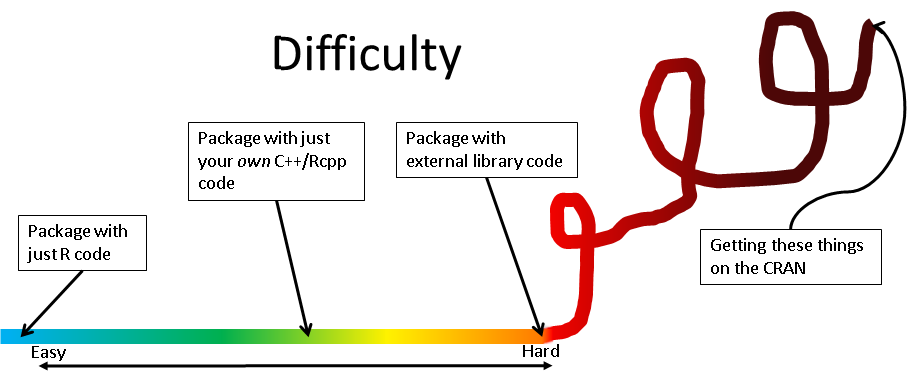
\includegraphics[scale=.55]{pics/packages}
\end{center}
\end{frame}

\begin{frame}{Getting on the CRAN}
\begin{center}
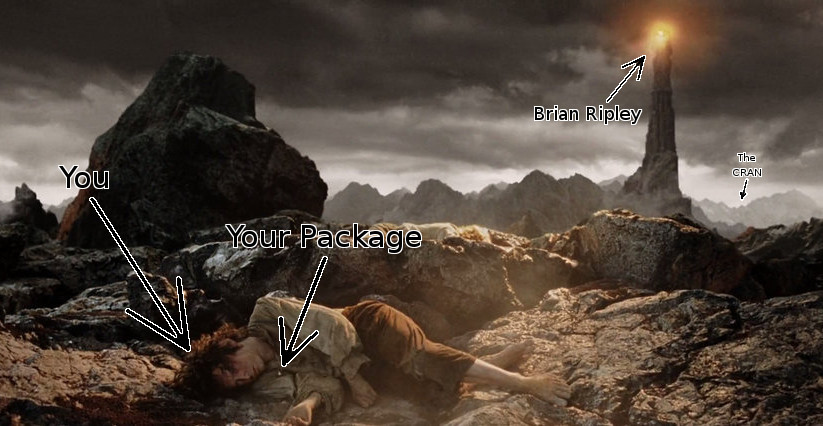
\includegraphics[scale=.46]{pics/cran_ripley}
\end{center}
\end{frame}
